\chapter{Preliminaries}
\label{ch:preliminaries}

In this project, some unsupervised algorithms can be used as the clustering model to extract the potential topics in the input documents. According to \cite{allahyari2017brief}, clustering, regarding as popular data mining algorithms, is extensively used in classification \cite{baker1998distributional, bekkerman2001feature} and document organization. However, some traditional clustering algorithms are not suited for text clustering because of some unique properties of text such as large dimensionality and the word correlation \cite{allahyari2017brief}. In this section, the two common types of text clustering algorithms, embedding-based clustering algorithms and probabilistic-based clustering algorithms, are demonstrated as the preliminaries of this project.

\section{Word-Embedding-Based Clustering Algorithm}

\subsection{Feature Extraction Techniques}
A simple way to implement text clustering is to extract the key features of the text and group the documents by traditional clustering algorithms such as K-means cluster. One-hot encoding, TF-IDF and word2vec are the most common strategies for text feature extraction. Using one-hot encoding on feature extraction is a kind of BOW (bag of word). The basic idea is to ignore the order of words and represent a document by the frequency of each word in the document. If the size of the dictionary is n and we want to represent a certain word is on k position, we can create an n-dimensionality vector, whose the k dimensionality would be set to 1 while the other would be set to 0. And the vector of the sample document can be expressed by directly added vectors of each word in the document. 

For example, there are two sentence: 1) This is an example. 2) This is another example. The dictionary of the above sentence is: {'this', 'is', 'a', 'another', 'example'}. The feature vector of sentence 1 is [1, 1, 1, 0, 1] and that of sentence 2 is [1, 1, 0, 1, 1].

TF-IDF is a common weighing technology for data mining and information retrieval \cite{mishra2015analysis}. TF means the term frequency, and the more frequently the term appears in the document, the larger TF value would be. As the following formula shows, ${n_{i,j}}$ is the count of word $i$ in document $j$ and the denominator is the sum of the number of occurrence of all words in the document ${d_{{j}}}$.

\begin{equation}
    {TF_{i,\ j}=\ \frac{n_{i,j}}{\sum_{k}n_{k,j}}}
\end{equation}

IDF means the inverse document frequency, and the less frequently the term appears in the corpus, the larger IDF value would be. The following is the calculation of IDF, where $|D|$ is the number of documents in the corpus and $\{j\ :\ t_i\ \in d_j\}$ means the number of documents which contain term $i$. The addition of 1 is to prevent the denominator being zero when the term $i$ is not in the corpus.

\begin{equation}
    IDF_i=\log{\frac{|D|}{\{j\ :\ t_i\ \in d_j\}\ +\ 1}}
\end{equation}

The value of TF-IDF can represent the importance of a term for the corpus, which can be calculate as the product of $TF_{i,j}$ and $IDF_i$

\begin{equation}
    {TF-IDF_{i,j}=TF_{i,\ j}\ \times IDF_i}
\end{equation}

Both one-hot encoding and TF-IDF are simple and fast ways to extract the text features, but they all focus on the frequency of the words and ignore the sequence of the words. It assumes that the word are independent of each other and neglect the mutual relation between the words. Additionally, the obtained features are discrete and sparse.

Since the shortage of the above techniques, word-embedding technique has been proposed. Word-embedding is a representation of word, and is technique that project words to real-number vectors, where words with similar meaning s have similar representations. Word2vec algorithm\cite{mikolov2013efficient, mikolov2013distributed}, as one of the word-embedding techniques, can learn the word associations by neural network from a large corpus \cite{enwiki:1006343323}. It use  Besides semantic similar words should be encoded into neighboring regions, expected word vectors should also support simple vector operations, which project semantic operations to vector operations. For example, $vec(king) + vec(woman) - vec(man) = vec(queen)$ \cite{church2017word2vec}. Moreover, to add the influence of context on the word rather than only analysis the text on word-dimensionality, doc2vec method was proposed by Le and T \cite{le2014distributed}. Doc2vec is based on word2vec method but adds a paragraph vector for training, which means that when training a sentence or a document, each time predicting the probability of the word, it uses the semantics of the entire sentence. 

\subsection{K-means Clustering}
After extracting features of text, clustering algorithms such as K-means cluster can be applied on them. K-means is a partitioning based algorithm proposed by McQUeen \cite{macqueen1967some}. The basic idea of K-means is that for a given sample set, it is expected to be divided into K clusters according to the distance between the samples and the centers. The points in each cluster are expected to be as closed as possible with each other and the distance among the clusters is expected to be large enough.

The main steps of K-means algorithm are as follows \cite{jain2010data}:

\begin{algorithm}[H]
  \SetAlgoLined
  \KwIn{Sample set}
  \KwOut{Clustered result}
  Random choose the initial centers of K clusters\;
  Initialize k samples as the initial cluster centers $a=a_1, a_2,...a_k$\;
  \While{cluster membership does not stabilize}{
  \For{each sample $x_i$}{
    Calculate the distance to each cluster center, and assign it to its closets center\;
 }
 \For{each cluster $a_j$}{
    Re-calculate and update its cluster center $a_j=\frac{1}{\vert c_i \vert}\sum_{x \in c_i} x$\;
 }
 }
  \caption{K-means algorithm}
\end{algorithm}

Additionally, in K-Means, Euclidean Metric or cosine distance is often used to calculate the distance between each sample.



\section{Probabilistic-Based Clustering Algorithm}
Topic modeling is a probability-based clustering tool for data mining and discovering the relationships in text documents \cite{allahyari2017brief, jelodar2019latent}. Traditional topic models such as Latent Semantic Index (LSI) and Probabilistic Latent Semantic Analysis (PLSA) have been applied in information retrieval, NLP, machine learning for text and related areas \cite{hofmann2013probabilistic}. Those algorithms assume each document is generated by repeating the steps that choosing a topic based on a certain probabilistic then choosing the word from the topic with a certain probabilistic. Combined with Bayesian probability framework, Latent Dirichlet Allocation (LDA) was proposed \cite{blei2003latent}, and a more advanced model Biterm Topic Model (BTM) is also produced based on LDA. The followings are the derivations of LDA and BTM \cite{heinrich2005parameter}.

\subsection{Mathematical Basis} \label{math}
To understand the principle of LDA and BTM, there are some mathematical basis should be known in advance. 

LDA proposed based on Bayesian model, and the basic process of Bayesian parameter estimation is 

   $$ prior\ distribution\ +\ data(likelihood)\ =\ posterior\ distribution$$

Using coin toss as an example, assume the probability of the coin being heads up is $p$, repeat $n$ times trials, the probability of $k$ times being heads up can be represented as a binomial distribution.

\begin{equation}
    Binom(k|n,p)\ =\ \binom{n}{k}p^k{(1-p)}^{n-k}
\end{equation}

To estimate the parameters, besides the likelihood, the prior and the posterior should also be known. Prior probability is a estimate probability before the event happen while the posterior probability is obtained by correcting the prior probability based on a certain evidence. In Bayesian probability theory, if the posterior distribution is the same as the prior probability distribution, the prior and posterior are called conjugate distribution \cite{enwiki:1013644991}. Regard the above binomial distribution as the likelihood, its conjugate distribution is Beta distribution. The general formula for Beta distribution is as follows:

\begin{equation}
    Beta(p|\alpha,\beta)\ =\ \frac{\Gamma(\alpha+\beta)}{\Gamma(\alpha)\Gamma(\beta)}p^{\alpha-1}{(1-p)}^{\beta-1}
\end{equation}

And the posterior probability distribution is :

\begin{equation}
\begin{aligned}
    P(p|n,k,\alpha,\beta)\ &\propto\ P(k|n,p)P(p|\alpha, \beta)\\
    &=\ P(k|n,p)P(p|\alpha,\beta)\\
    &=\ Binom(k|n,p)Beta(p|\alpha,\beta)\\
    &=\ \binom{n}{k}p^k{(1-p)}^{n-k}\times \frac{\Gamma(\alpha+\beta)}{\Gamma(\alpha)\Gamma(\beta)}p^{\alpha-1}{(1-p)}^{\beta-1} \\
    &\propto\ p^{k+\alpha -1}{(1-p)}^{n-k+\beta -1}
\end{aligned}
\end{equation}

Normalization the above equations, the posterior probability is as follows, and the posterior probability distribution is exactly the Beta distribution.

\begin{equation}
    P(p|n,k,\alpha,\beta)\ =\ \frac{\Gamma(\alpha+\beta+n)}{\Gamma(\alpha+k)\Gamma(\beta+n-k)}p^{k+\alpha-1}{(1-p)}^{n-k+\beta-1}
\end{equation}

Therefore, the intuitive expression of the above Bayesian analysis process is:

\begin{equation}
    Beta(p|\alpha,\beta)\ +\ BinomCount(k, n-k)\ =\ Beta(p|\alpha+k, \beta+n-k)
\end{equation}

Extend the above two-dimensional process to multi-dimensional. The multinomial distribution is the extension of the binomial distribution, and Dirichlet distribution is the conjugate prior of multinomial distribution, which is also the multivariate generalization of the Beta distribution \cite{lin2016dirichlet}.

Assume still do $n$ times trials, each time has $m$ results, the multinomial distribution is $multi(\vec m|n, \vec p)$. $\vec \alpha\ =\ (\alpha_1,\alpha_2,...,\alpha_k)$ is the parameter of the Dirichlet distribution, the Dirichlet distribution can be represented as $Dirichlet(\vec p|\vec \alpha)$. The same as Beta-Binomial conjugate, Dirichlet-Multinomial conjugate can be described as:

\begin{equation}
    Dirichlet(\vec p|\vec \alpha)\ +\ MultiCount(\vec m)\ =\ Dirichlet(\vec p|\vec \alpha+\vec m)
\end{equation}

Additionally, for a nature of Dirichlet distribution, the mathematical expectation of the distribution $\vec p\ \sim\ Dir(\vec t|\vec\alpha)$ is:

\begin{equation}\label{expectation}
    \mathbb{E}(\vec p)\ =\ (\frac{\alpha_1}{\sum_{i=1}^{K}\alpha_i}, \frac{\alpha_2}{\sum_{i=1}^{K}\alpha_i},..., \frac{\alpha_K}{\sum_{i=1}^{K}\alpha_i},)
\end{equation}

\subsection{LDA}
As claimed in \cite{blei2003latent}, LDA is proposed as a generative probabilistic model for collecting discrete data. 
The physical process of LDA text modeling can be described as a dice game.  

\begin{algorithm}[H]
  There are two jars contains doc-topic dices and topic-word dices respectively\;
  Randomly pick $K$ topic-word dices and number them from 1 to $K$\;
  Before generating a new document, randomly pick a doc-topic dice, and repeat the following steps to generate the words in the document\;
  \Repeat{finish the document}{
    Throw this doc-topic dice and get a topic $z$\;
    Pick the number $z$ dice from $K$ topic-word dices, then throw it to get a word\;
  }
  \caption{LDA Topic Model}
\end{algorithm}

Assume there are $M$ documents in the corpus, all the word and their topics in the document can be denoted as vectors, in which $\vec w_m$ denote the words in the $m^{th}$ document and $\vec z_m$ denote the corresponding topics of the words. 

$$\vec w\ =\ (\vec w_1,...,\vec w_M)$$
$$\vec z\ =\ (\vec z_1,...,\vec z_M)$$

% \begin{figure}[H]
%     \centering
%     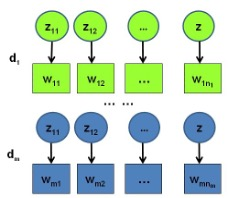
\includegraphics[scale=0.8]{images/words&topics.jpg}
%     \caption{Words and Topics}
%     \label{fig:5}
% \end{figure}

The figured process of LDA model is as figure \ref{fig:5} shows. $\vec \theta_m$ in the doc-topic dice and $\vec \varphi_k$ in the topic-word dice are the parameters in the model, which correspond to multinomial distribution. 

\begin{figure}[H]
    \centering
    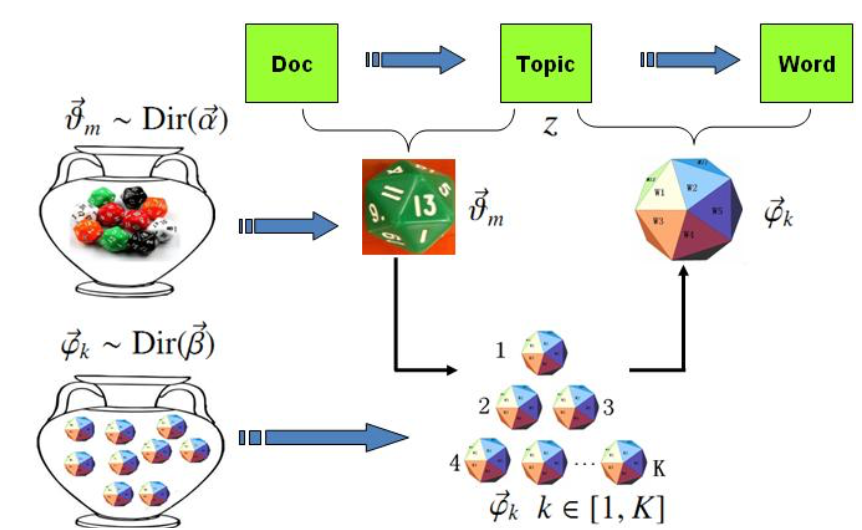
\includegraphics[scale=0.6]{images/LDA_model.png}
    \caption{LDA Model \cite{jin_2013}}
    \label{fig:5}
\end{figure} 

% \begin{figure}[H]
%     \begin{minipage}[t]{0.6\linewidth}
%         \centering
%         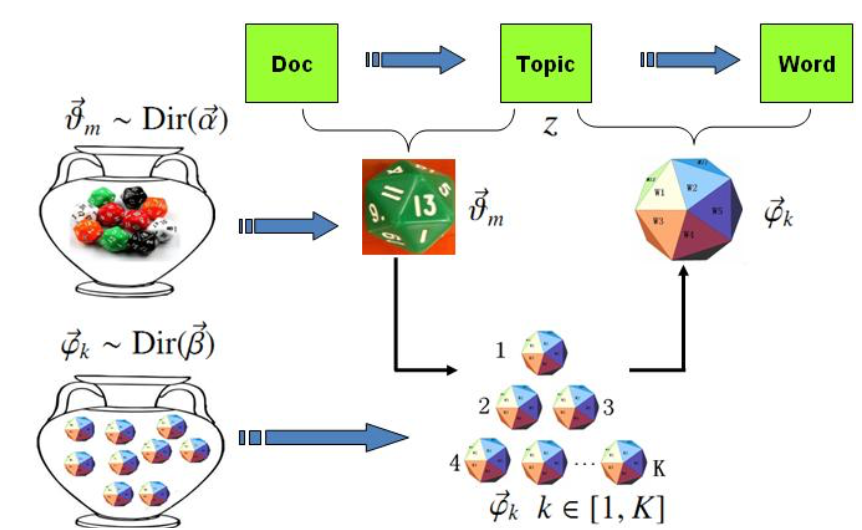
\includegraphics[scale=0.6]{images/LDA_model.png}
%         \caption{LDA Model}
%         \label{fig:7}
%     \end{minipage}%
%     \begin{minipage}[t]{0.3\linewidth}
%         \centering
%         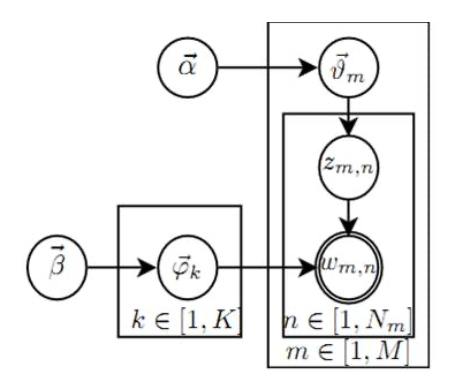
\includegraphics[scale=0.8]{images/graph_lda.png}
%         \caption{Probabilistic Graphic Model of LDA}
%         \label{fig:8}
%     \end{minipage}
% \end{figure}


Figure \ref{fig:6} is the probabilistic graphic model of LDA. It can be broken down to two physical processes:

\begin{enumerate}
    \item $\vec \alpha\ \rightarrow\ \vec \theta_m\ \rightarrow\ z_{m,n}$, denotes the process that when generating the $m^{th}$ document, pick a doc-topic dice $\vec \theta_m$, then use this dice to generate the topics $z_{m,n}$ of the $n^{th}$ word;
    
    \item $\vec \beta\ \rightarrow\ \vec\varphi_k\ \rightarrow\ w_{m,n}|k\ =\ z_{m,n}$, denotes the process using the dice numbered $k\ =\ z_{m,n}$ from $K$ topic-word dices $\vec \varphi_k$ to generate the word $w_{m,n}$, which means generate the $n^{th}$ word in the $m^th$ document.
\end{enumerate}

\begin{figure}[H]
    \centering
    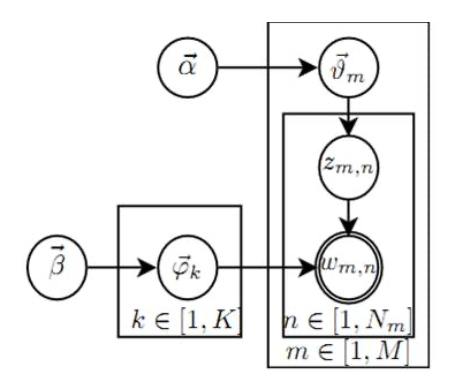
\includegraphics[scale=0.8]{images/graph_lda.png}
    \caption{Probabilistic Graphic Model of LDA \cite{jin_2013}}
    \label{fig:6}
\end{figure}

For the first process, $\vec \alpha\ \rightarrow\ \vec\theta_m$ corresponds to Dirichlet distribution and $\vec\theta_m\ \rightarrow\ \vec z_m$ corresponds to Multinomial distribution. Thus, this process is a conjugate structure:

    $$\vec\alpha \underbrace{\ \longrightarrow\ }_{Dirichlet} \vec\theta \underbrace{\ \longrightarrow\ }_{Multinomial} \vec z_m$$

Based on little computing, we can get:

$$p(\vec z_m|\vec\alpha)\ =\ \frac{\Delta(\vec n_m+\vec\alpha)}{\Delta(\vec\alpha)}$$

in which $\vec n_m\ =\ (n_m^{(1)},...,n_m^{(k)}))$, $n_m^{(k)}$ is the number of words that generated from $k^{th}$ topic. Moreover, utilizing the Dirichlet-Multinomial conjugate, the posterior distribution of parameter $\vec\theta_m$ is:

$$Dir(\vec\theta_m|\vec n_m+\vec\alpha)$$

The generations of topics of $M$ documents are independent, thus there are $M$ independent Dirichlet-Multinomial structures. And the probability of the topic generation is:

\begin{equation}\label{pza}
\begin{aligned}
    p(\vec z|\vec\alpha)\ &=\ \prod_{m=1}^{M}p(\vec z_m|\vec\alpha)\\
    &=\ \prod_{m=1}^{M}\frac{\Delta(\vec n_m+\vec\alpha)}{\Delta(\vec\alpha)}
\end{aligned}
\end{equation}

Similarly, for the second process $\vec\beta\ \rightarrow\ \vec\varphi_k\ \rightarrow\ \vec w_{(k)}$, $\vec\beta\ \rightarrow\ \vec\varphi_k$ corresponds to Dirichlet distribution and $\vec\varphi_k\ \rightarrow\ \vec w_{(k)}$ corresponds to Multinomial distribution:

   $$\vec\beta \underbrace{\ \longrightarrow\ }_{Dirichlet} \vec\varphi_k \underbrace{\ \longrightarrow\ }_{Multinomial} \vec w_{(k)}$$

Based on the computing and this conjugate structure, the posterior distribution of parameter $\varphi_k$ is also a Dirichlet distribution $Dir(\vec\varphi_k|\vec n_k+\vec\beta)$. The generations of words from $K$ topics in the corpus are independent from each other, thus there are $K$ independent Dirichlet-Multinomial conjugate structures. And the probability of the generation of the words in the whole corpus is \cite{heinrich2005parameter}:

\begin{equation}\label{pwz}
\begin{aligned}
    p(\vec w|\vec z, \vec\beta)\ &=\ p(\vec w^{'}|\vec z^{'}, \vec\beta)\\
    &=\ \prod_{k=1}^{K}p(\vec w_{(k)}|\vec z_{(k)}\vec\beta)\\
    &=\ \prod_{k=1}^{K}\frac{\Delta(\vec n_k+\vec\beta)}{\Delta(\vec\beta)}
\end{aligned}
\end{equation}

Combined equation \ref{pza} with \ref{pwz}, the probability of the generation of the whole corpus is \cite{heinrich2005parameter}:

\begin{equation}
\begin{aligned}
    p(\vec w,\vec z|\vec\alpha,\vec\beta)\ &=\ p(\vec w|\vec z,\vec\beta)p(\vec z|\vec\alpha)\\
    &=\ \prod_{k=1}^{K}\frac{\Delta(\vec n_k+\vec\beta)}{\Delta(\vec\beta)}\ \prod_{m=1}^{M}\frac{\Delta(\vec n_m+\vec\alpha)}{\Delta(\vec\alpha)}
\end{aligned}
\end{equation}

With the joint distribution $p(\vec w,\vec z)$, Gibbs sampling can be used to estimate the posterior distribution by collecting the samples \cite{hrycej1990gibbs}. Gibbs sampling is a Markov chain Monte Carlo (MCMC) algorithm used when direct sampling is difficult\cite{enwiki:992631521}, which is regarded as a simulation tool to acquire samples from non-normalized joint density function\cite{gelfand2000gibbs}.

The $\vec w$ is the observed known data, while $\vec z$ is the implicit variable. Thus, the distribution that should be sampled is $p(\vec z|\vec w)$. Mark the topic of the $i^{th}$ word in corpus $\vec z$ as $z_i$, where $i\ =\ (m,n)$ and corresponds to the $n^{th}$ word in the $m^{th}$ document and $\lnot i$ means get rid of word $i$. According to the requirement of Gibbs sampling algorithm, we should get the corresponding condition distribution $p(z_i=k|\vec z_{\lnot i},\vec w)$ of each arbitrary coordinate axis $i$. After getting rid of the $i^{th}$ word, the Dirichlet-Multinomial conjugate will not be changed. Thus, the posterior distribution of both $\vec\theta_m$ and $\vec\varphi_k$ still are Dirichlet distribution:

    \begin{equation}\label{parameters}
    \begin{split}
        p(\vec\theta_m|\vec z_{\lnot i},\vec w_{\lnot i})\ &=\ Dir(\vec\theta_m|\vec n_{m, \lnot i}+\vec\alpha)\\
        p(\vec\varphi_k|\vec z_{\lnot i},\vec w_{\lnot i})\ &=\ Dir(\vec\varphi_k|\vec n_{k, \lnot i}+\vec\beta)
    \end{split}
    \end{equation}

Assume the observed word $w_i=t$, based on the Bayesian rule(the conditional probability is proportional to joint probability) and combined with the above equation \ref{parameters} \cite{heinrich2005parameter}:

\begin{equation}
\begin{aligned}
    p(z_i=k|\vec z_{\lnot i},\vec w)\ &\propto\ p(z_i=k,w_i=t|\vec z_{\lnot i},\vec w_{\lnot i})\\
    &=\ \mathbb{E}(\theta_{mk})\ \cdot\ \mathbb{E}(\varphi_{kt})\\
    &=\ \hat{\theta}_{mk}\ \cdot\ \hat{\varphi}_{kt}
\end{aligned}
\end{equation}

Additionally, knowing the posterior distribution, the way to estimate the parameter is to use the mean value of this parameter in the posterior distribution. The expectation of Dirichlet distribution, as equation \ref{expectation}, can estimate each parameter $\hat{\theta}_{mk}$ and $\hat{\varphi}_{kt}$ \cite{heinrich2005parameter}:

\begin{equation}
\begin{split}
    \hat{\theta}_{mk}\ &=\ \frac{n_{m,\lnot i}^{(k)}+\alpha_k}{\sum_{k=1}^{K}(n_{m,\lnot i}^{(k)}+\alpha_k)}\\
    \hat{\varphi}_{kt}\ &=\ \frac{n_{k,\lnot i}^{(t)}+\beta_t}{\sum_{t=1}^{V}(n_{k,\lnot i}^{(t)}+\beta_t)}
\end{split}
\end{equation}

The final Gibbs sampling formula for LDA model is as follows, in which the right side is $p(topic|doc)\ \cdot\ p(word|topic)$. This Gibbs sampling can help to sample the topics of all the words in the corpus. And the Gibbs sampling algorithm can be used to train or inference the LDA model.

\begin{equation}
    p(z_i=k|\vec z_{\lnot i},\vec w)\ \propto\ \frac{n_{m,\lnot i}^{(k)}+\alpha_k}{\sum_{k=1}^{K}(n_{m,\lnot i}^{(k)}+\alpha_k)}\ \cdot\ \frac{n_{k,\lnot i}^{(t)}+\beta_t}{\sum_{t=1}^{V}(n_{k,\lnot i}^{(t)}+\beta_t)}
\end{equation}

% The right side of the formula is $p(topic|doc)\ \cdot\ p(word|topic)$. Since there are $K$ topics, the physical meaning of this Gibbs sampling formula is sample the $K$ path.

% 训练和inference过程写在design里

\subsection{BTM}
The main difference between BTM and LDA is that LDA modeling each word in the corpus while BTM modeling each biterms. 'biterm' denotes the word pair co-occuring in the text\cite{cheng2014btm}. For example, document $(w_1, w_2, w_3)$ will generate three biterms $\{(w_1,w_2), (w_1,w_3), \\(w_2,w_3)\}$. The formula derivation of BTM is basically the same as LDA. The difference of LDA and BTM is showed as the graphical representation figure \ref{fig:7}

\begin{figure}[H]
    \begin{minipage}[t]{0.5\linewidth}
        \centering
        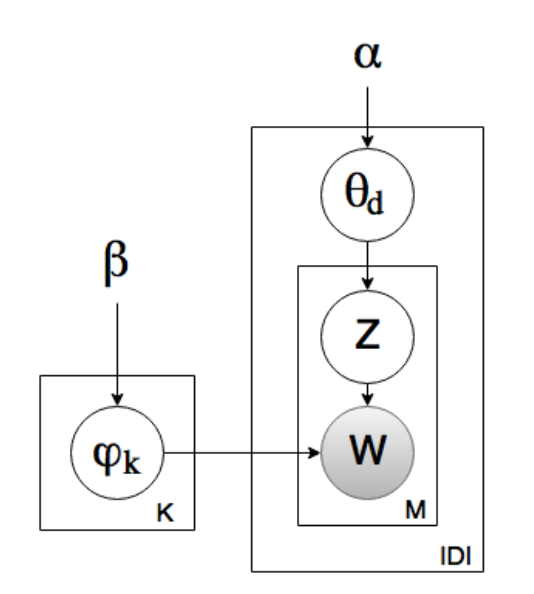
\includegraphics[scale=0.5]{images/LDA.png}
        % \caption{LDA}
        % \label{fig:7}
    \end{minipage}%
    \begin{minipage}[t]{0.5\linewidth}
        \centering
        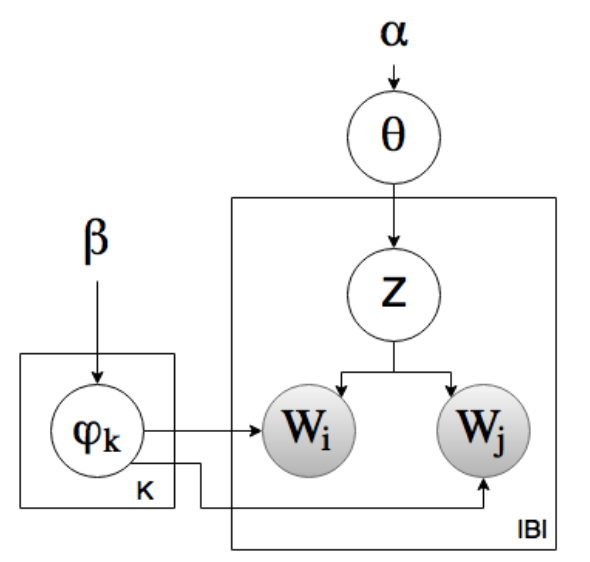
\includegraphics[scale=0.5]{images/BTM.png}
        % \caption{Graphical representation of BTM}
        % \label{fig:8}
    \end{minipage}
    \label{fig:7}
    \caption{Graphical representation of LDA(left) \& BTM(right)  \cite{jonsson2015evaluation}}
\end{figure}

The generation of the corpus in BTM is described as follows\cite{cheng2014btm}:

\begin{enumerate}
    \item Draw $\theta\sim Dirichlet(\alpha)$
    \item For each topic $k\in[1,K]$
    \begin{enumerate}
        \item draw $\phi_k\sim Dirichlet(\beta)$
    \end{enumerate}
    \item For each biterm $b_i\in B$
    \begin{enumerate}
        \item draw $z_i\sim Multinomial(\theta)$
        \item draw $w_i,w_j\sim Multinomial(\phi_{z_i})$
    \end{enumerate}
\end{enumerate}

Assume the $i^{th}$ biterm in the corpus as $b_i=\{w_i,w_j\}$, in which the words $w_i=t_1$, $w_j=t_2$. $z_{\lnot i}$ denotes the topics for all biterms except $b_i$, $n_{\lnot i}^{(k)}$ is the number of biterms assigned to topic $k$ except $b_i$, and $n_{\lnot i,k}^{(w)}$ denotes the number of times that word $w$ assigned to topic $k$ except words in $b_i$ \cite{cheng2014btm}. The extend of the Gibbs sampling formula for BTM is:
\begin{equation}
\begin{aligned}
    p(z_i=k|\vec z_{\lnot i},\vec b)\ &\propto\ \theta_k\ \cdot\ \varphi_{k, w_i}\ \cdot\ \varphi_{k,w_j}\\
    &=\ \frac{n_{\lnot i}^{(k)}+\alpha_k}{\sum_{k=1}^{K}(n_{\lnot i}^{(k)}+\alpha_k)}\ 
    \cdot\ \frac{n_{\lnot i,k}^{(t_1)}+\beta_{t_1}}{\sum_{t_1=1}^{V}(n_{\lnot i,k}^{(t_1)}+\beta_{t_1})}\ 
    \cdot\ \frac{n_{\lnot i,k}^{(t_2)}+\beta_{t_2}}{\sum_{t_2=1}^{V}(n_{\lnot i,k}^{(t_2)}+\beta_{t_2})}
\end{aligned}
\end{equation}

